%describe the tasks to be completed that will satisfy the given objective
\section{Activity}
Useful and/or necessary background knowledge is first provided in the Theory section, followed by more detailed instructions in the Implementation section.

\subsection{Theory}
Refer to this section and subsections as needed during your implementation (see below) of the solution.

\subsubsection{Fast Fourier Transform}
The \ac{fft} is a special case of the more general Fourier transform in that the \ac{fft} only applies to discrete data.
The \ac{fft} has various applications, but the application for which it will be used here is to decompose an audio waveform into its constituent frequencies.
A full discussion of the Fourier transform is beyond the scope of this lab and this course, but some examples of it in action will be given.
Please note that these examples are meant to illustrate concepts rather than be perfectly accurate in their results.
Figure~\ref{fig:cft} demonstrates the result of a continuous Fourier transform applied upon a sine wave.
\begin{figure}[h]
\centering
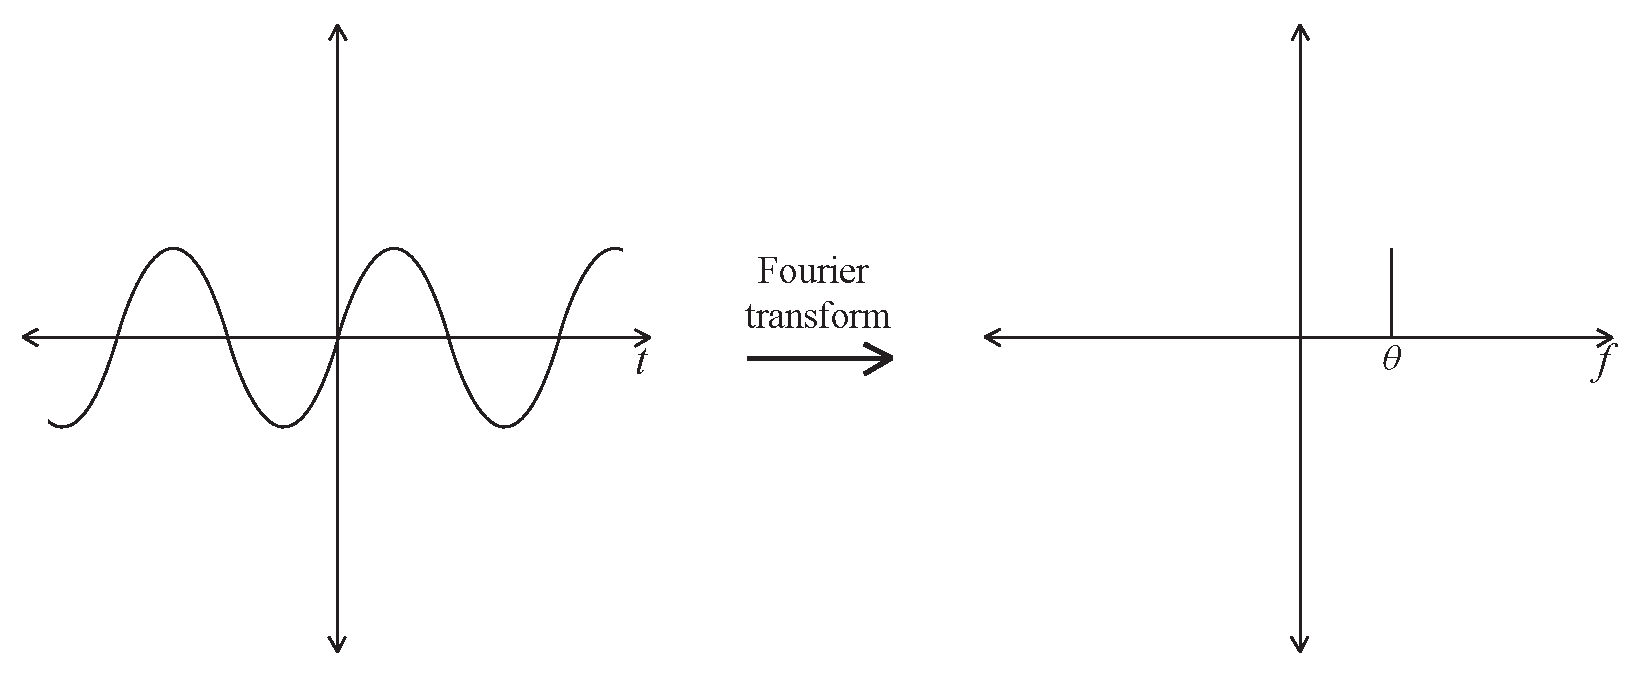
\includegraphics[width=0.8\textwidth]{CFT.pdf}
\caption{The Fourier transform of a sine wave with frequency $\theta$ in the time domain results in a single peak in the frequency domain at $\theta$.}
\label{fig:cft}
\end{figure}
Figure~\ref{fig:dft} on the other hand illustrates the expected results of a discrete Fourier transform applied upon a discretized sine wave.
\begin{figure}[h]
\centering
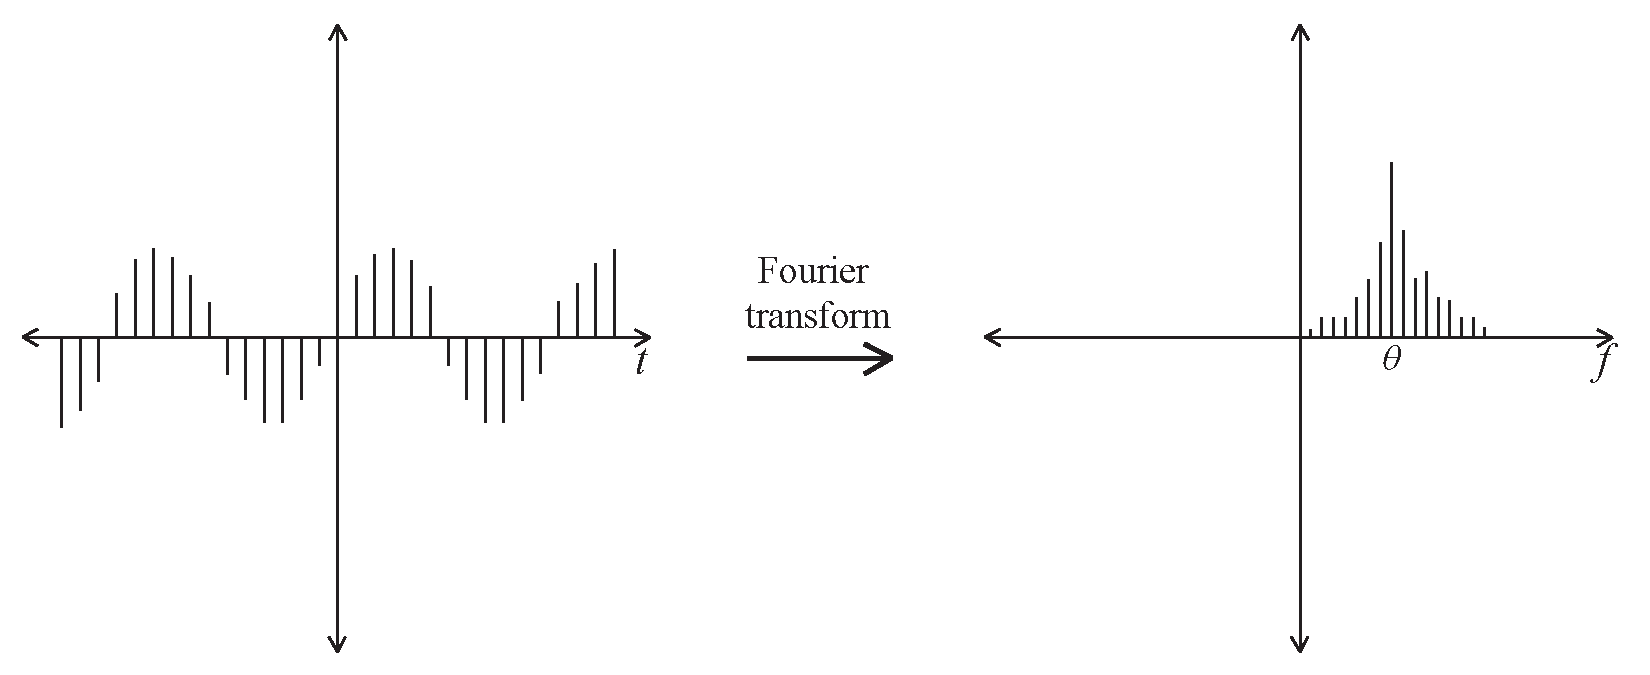
\includegraphics[width=0.8\textwidth]{DFT.pdf}
\caption{The Fourier transform of discrete samples approximating a sine wave with frequency $\theta$ in the time domain results in a rough distribution in the frequency domain peaked at (or near) $\theta$.}
\label{fig:dft}
\end{figure}
As you can see, the frequency decomposition is not as well-defined in the discrete case.
Instead, frequencies are divided into bins of constant width, each with an associated magnitude (the peaks in Figure~\ref{fig:dft}).
This lack of definition is due to the fact that the information given is incomplete and noisy (error prone).
If you were to increase the number of samples taken, the frequency decomposition would expectedly become cleaner (the bins become smaller).
However, taking more samples has a drawback in that it takes longer to collect and process them.
The continuous case is basically the result of extending this thought and taking an infinite amount of samples.
Since we can't take an infinite amount of samples, we will just have to settle with the rough peak in the discrete transform.

In Java, the \ac{fft} is implemented as a \verb=static= function of the {\tt FastFourierTransform} class.
It takes an array of \verb=Complex= objects as input, and places its output into the given array.
This means that once you give it something, the input is lost (unless you want to implement the Inverse \ac{fft}).

The \verb=Complex= objects the \ac{fft} takes as arguments are simply representations of complex numbers $a+bi$, where $a$ is the real part and $b$ is the imaginary part.
Complex numbers are intimately related to waves and the \ac{fft}, but the only extent to which you need to understand them is very basic.
As long as you can perform the operations of complex addition, subtraction, multiplication, and division, you should be fine.
The \verb=FastFourierTransform= and \verb=Complex= classes are provided for you in the package {\tt csc120.lab6.FFT}.

\subsubsection{Musical Scales}
There are many ways to define a musical scale, and ultimately all of them are arbitrary.
We will assume that we are using the equal temperament chromatic scale.
In this scale, there are 12 notes in an octave, with an octave merely an ordered collection of notes before they start over.
That is, each octave contains the same 12 notes.
The notes are in order as follows: C, C\#, D, D\#, E, F, F\#, G, G\#, A, A\#, B, with \# pronounced ``sharp."
The standard American scale is based upon the note A 440, which is the A note, 4th octave, at 440 Hz.
Each octave is a factor of 2 larger or smaller than the next or previous (A3 is 220 Hz and A5 is 880 Hz).
In addition, each note is evenly spread out in an octave in equal temperament, such that every note is a constant factor away from its neighbors.
Since we are on a 12 note scale, this constant factor is the twelfth root of two, $ \sqrt[12]{2}$.

\subsection{Implementation}
There are several tasks that you must complete in order to have a functional tuner. 
These tasks need not be completed in any specific order, though they are presented in the order of their logical flow from one part of the problem to the next.

\subsubsection{Research}
You may wish to look up the usage of the following Java keywords or operators if you have not seen them before: \verb=static=, modulo, and casting.
A resource declared with the \verb=static= keyword is accessible even if there is no object declared.
The modulo operator (\%) returns the remainder of a division operation.
Casting converts one data type to another and is useful in avoiding truncation of integers, e.g. \verb+double d = (double) 5 / (double) 7+.

\subsubsection{Implement Complex Numbers}
Though the \verb=Complex= class has been provided, it is not completely implemented.
Before the \ac{fft} will work, you must provide the implementation for the following functions: \verb=plus()=, \verb=minus()=, \verb=times()=, and \verb=dividedBy()=.
Each function takes a \verb=Complex= parameter and returns a \verb=Complex= argument such that \verb=A.plus(B)= equals the sum of two complex numbers A and B.
As a hint for the division of two complex numbers, consider multiplying the numerator and denominator of the fraction 
\begin{math}
(a+bi) / (c+di)
\end{math} 
 by the conjugate of the denominator, $c-di$.

\subsubsection{Get the Audio Data}
The results of this section should belong in the \verb=SoundAnalyzer.onHandleIntent()= function provided.
Audio can be retrieved from the microphone by using the \verb=AudioRecord= class.
Class methods of particular interest are \verb=startRecording()=, \verb=read()=, \verb=stop()=, and \verb=release()=.
The \verb=AudioRecord= object should be constructed to read 16 bit PCM mono audio at a rate of 44.1 kHz into an array of shorts.
The size of this array should be a power of 2 (4096 is recommended).
For further information, refer to the Android API and other internet resources.

\subsubsection{Obtain the Frequency Decomposition}
This section's contents should also belong in the \verb=SoundAnalyzer.onHandleIntent()= function.
After obtaining the array of audio shorts, these should be converted into the real components of an array of \verb=Complex= objects (with imaginary components of zero).
This \verb=Complex= array should then be passed to the function \verb=FastFourierTransform.fft()=.
The results of the \ac{fft} are contained in the same array.
Each index of the output array corresponds to a frequency, and the \verb=Complex= object at an index measures the magnitude of that frequency in the audio signal.
In other words, the indices map to the locations of the peaks on the right sides of Figures~\ref{fig:cft} and~\ref{fig:dft}, and the magnitudes map to the heights of the peaks.
An index maps to a frequency according to the following formula: $frequency = index*sampleRate/arraySize$.
A \verb=Complex= object maps to a magnitude according to the following formula: $magnitude = \sqrt{a^2 + b^2}$.

\subsubsection{Choose a Representative Frequency}
Again, this task should be confined to the \verb=SoundAnalyzer.onHandleIntent()= function.
There are many methods one could use to determine the representative frequency.
We will use what is arguably the simplest: pick the frequency of maximum magnitude.
You will want to hold onto this value for later.

\subsubsection{Implement the Musical Scale}
It is required that you implement the musical scale in its own class.
The class should provide a function that finds the nearest note to a given frequency as well as a function that calculates the frequency of a desired note.
The first 10 octaves are sufficient to cover the entire range of human hearing.

\subsubsection{Choose the Reference Note}
This task can logically be contained within the \verb=TunerActivity.tune()= function.
Use the musical scale that you have constructed to find the nearest note to your representative frequency.
Note that since each successive octave is twice the size of the previous and the gap between notes gets larger and larger, simply finding the closest note to your estimated fundamental may not be sufficient in all cases.
You may consider using a log scale of the frequencies to address this issue.

\subsubsection{Inform the User}
Make a call to the \verb=TunerActivity.updateGUI()= function inside of \verb=TunerActivity.tune()=.
The parameters in order are as follows: the note with octave (e.g. C\#4),  the estimated representative frequency, how far below the note the frequency is (on a scale of 0 to 100), and how far above the note the frequency is (same scale as previous).
If the frequency is either above or below the note, then the third or fourth parameter should be zero, respectively.

\subsubsection{Debug}
At some point you will undoubtedly wish to test your solution for correctness.
There are several resources you could use, including YouTube videos (search ``a 440") and actual instruments.
The most appropriate resource can be found at http://ptolemy.eecs.berkeley.edu/eecs20/week8/frequencylive.html.
Do not be concerned if your tuner is not 100\% accurate, fails on complex tones, or indicates that a note is slightly off when you know otherwise; these are consequences of the method we used to choose the representative frequency.

\subsubsection{Optional Refinements}
If you would like to improve the functionality of your tuner, there are two primary avenues that you could follow.
The first is to research alternate methods to choose the representative frequency.
These methods may consist of advanced topics such as interpolation or harmonic analysis.
The second route is to supplement your existing program by filtering ambient noise (i.e. setting a minimum magnitude threshold).
The \verb=TunerActivity.tare()= function and button are provided for this purpose.

